
\documentclass[11pt,a4paper]{report}		                                   

\usepackage{a4}
%\usepackage{german}

%Deutsche Trennungen, Anführungsstriche, Rechtschreibung und mehr:
%-------------------------------------------------------------------
%\usepackage{german, ngerman}	% Trennungen, Anführungsstriche, ...
\usepackage[ngerman]{babel}		% Rechtschreibung
\usepackage[T1]{fontenc}        % Silbentrennung und Eingabe von Wörtern mit Umlauten

% Optionen zur Texteingabe und zum Darstellungsstil
%-------------------------------------------------------------------
\usepackage[utf8]{inputenc}			% Kodierung festlegen, für UTF-8 Unterstützung
\usepackage{lmodern}				% Benutze skalierbare Schriftfamilie
\usepackage[activate]{microtype}	% Verbesserte Darstellung der Schriftzeichen und
									% Zwischenräumen

% Zitierung und Literaturverzeichnis
%-------------------------------------------------------------------
%\usepackage{cite}
\usepackage[backend=bibtex,style=numeric]{biblatex}
\usepackage{csquotes}
\addbibresource{references.bib}

% Grafiken
%-------------------------------------------------------------------
\usepackage{graphicx}		% Zum Einbinden von Grafiken
\usepackage{wrapfig}		% Grafiken mit umfliessenden Text
\usepackage{subcaption}
%\usepackage{subfig}
\usepackage{float}			% Erlaubt Textumschlossene Bilder und Tabellen
\usepackage{tikz}			% Einbinden von Latexgrafiken

% Tabellen
%-------------------------------------------------------------------
\usepackage{multirow}		% Zusammenfassen von Zellen in Tabellen ermöglichen
\usepackage{tabularx}

% Links
%-------------------------------------------------------------------
\usepackage[pdfstartview=FitV, 	% start in 'fit size height'-view
			colorlinks=true, 	% Links farbig markieren
			linkcolor=black, 	% Interne Links schwarz
			citecolor=black, 	% Links zur Literatur schwarz
			filecolor=black, 	% Links auf lokale Dateien schwarz
			urlcolor=blue,   	% Externe Links blau
			breaklinks=true, 	% Links umbrechen
			linktocpage=false 	% Im Inhaltsverzeichnis sind Seitenzahlen UND Text Links
			]{hyperref}

% Einbettung von Code (C/C++, Java, ...)
%-------------------------------------------------------------------
%\usepackage{verbatim}		% Sorgt dafür, dass Text so dargestellt wird wie er eingegeben ist,
                            % es werden keine Leerzeichen oder Tabs entfernnt
%\usepackage{moreverb}		% Erweiterte Möglichkeiten für verbatim                            
\usepackage{courier}
\usepackage{listings}		% Source-Code printer for LaTeX
\lstset{language=Java}  	% Java
\lstset{numbers=left, numberstyle=\tiny, numbersep=-6pt,tabsize=3, stepnumber=1}
\lstset{framexleftmargin=-5mm, frame=single, rulesepcolor=\color{gray}}
\lstset{captionpos=b} 							% Beschriftung unter Listing
\lstset{backgroundcolor=\color[gray]{0.93}}
%\lstset{basicstyle=\scriptsize} 				% alle listings winzig drucken 
\lstset{basicstyle=\footnotesize\ttfamily, breaklines=true}
\lstset{commentstyle=\color[RGB]{63,127,80}}		% Kommentare gruen drucken 
\lstset{keywordstyle=\color{blue}\bfseries}		% Schlüsselwörter fett und blau

%sonstiges
%-------------------------------------------------------------------
\usepackage{todonotes}

\newcommand{\thema}{Automatisierte Implementierung interner Java-DSLs}
\newcommand{\schlagworte}{interne DSL, Java, Automatisierung, Code-Generierung}
\newcommand{\zusammenfassung}{Diese Masterarbeit behandelt die teilweise automatisierte Implementierung interner Java-DSLs. Die Grundlage einer Domänenspezifischen Sprache bildet dabei eine Anzahl von Interfaces, welche die Grammatik der Sprache definieren. Aus ihnen werden Teile der Sprach-Implementierung automatisch generiert. Die am besten geeigneten Datenstrukturen werden durch eine vorangehende manuelle Implementierung ermittelt. Ein besonderer Fokus wird auf die Trennung von Sprache und Implementierung gelegt. Dies verspricht für beide Teile hohe Wartbarkeit, Modularität und Wiederverwertbarkeit. Die daraus resultierenden Erkenntnisse werden in einen Code-Generator umgesetzt. Die angestrebte vollständige Trennung wird aus zeitlichen Gründen nicht erreicht, kann aber nachträglich ergänzt werden.}
\newcommand{\ausgabedatum}{19.10.2015}
\newcommand{\abgabedatum}{04.05.2016}
\newcommand{\autor}{Daniel Fritz}
\newcommand{\autorStrasse}{Dacherstra\ss e 1}
\newcommand{\autorPLZ}{78462 }
\newcommand{\autorOrt}{Konstanz}
\newcommand{\autorGeburtsort}{Konstanz}
\newcommand{\autorGeburtsdatum}{03.11.1987 }
\newcommand{\prueferA}{Prof. Dr. Heiko von Drachenfels}
\newcommand{\prueferB}{Prof. Dr. Oliver Eck}
\newcommand{\firma}{HTWG Konstanz}
\newcommand{\studiengang}{Master of Science Informatik}




\begin{document}

	
\begin{titlepage}

\vspace*{-3.5cm}

\begin{flushleft}
\hspace*{-1cm} 
\includegraphics[width=15.7cm]{htwg-logo}
\end{flushleft}

\vspace{2.5cm}

\begin{center}
	\huge{
		\textbf{\thema} \\[5cm]
	}
	\Large{
		\textbf{\autor}} \\[6.5cm]
	\large{
		\textbf{Konstanz, \abgabedatum} \\[2.3cm]
	}
	
	\Huge{
		\textbf{{\sf MASTERARBEIT}}
	}
\end{center}

\end{titlepage}

	\thispagestyle{empty}
{
\setlength{\parskip}{0.5cm}
        \begin{center}
        \textbf{\huge MASTERARBEIT}

        \textbf{zur Erlangung des akademischen Grades}

        \textbf{\Large Master of Science (M. Sc.)}

        \textbf{an der}

        \textsf{\huge Hochschule Konstanz}\\
        {\small Technik, Wirtschaft und Gestaltung}

        \textsf{\Large Fakultät Informatik} \\
        Studiengang \studiengang
        \end{center}
}
\begin{center}

\vspace*{2cm}

\begin{tabular}{p{3cm}p{10cm}}
Thema: & \textbf{\large \thema} \\[15ex]
Masterkandidat: & \autor, \autorStrasse, \autorPLZ  \autorOrt \\[15ex]
1. Prüfer: & \prueferA \\
2. Prüfer: & \prueferB \\[25ex]
Ausgabedatum: & \ausgabedatum \\
Abgabedatum: & \abgabedatum \\
\end{tabular}
\end{center}
	
\begin{center}
{\Large \textbf{Zusammenfassung (Abstract)}}
\end{center}

\bigskip

\begin{center}
	\begin{tabular}{p{2.8cm}p{10cm}}
		Thema: & \thema \\
		 & \\
		Masterkandidat: & \autor \\
		 & \\
		Firma: & \firma \\
		 & \\
		Betreuer: & \prueferA  \\[.5ex]
		 &  \prueferB \\
		 & \\
		Abgabedatum: & \abgabedatum \\
		 & \\
		Schlagworte: & \schlagworte \\
		 & \\
	\end{tabular}
\end{center}

\bigskip

\noindent
\zusammenfassung
	\chapter*{Ehrenwörtliche Erklärung}
\addcontentsline{toc}{chapter}{Ehrenwörtliche Erklärung}

Hiermit erkläre ich,
\textit{\autor, geboren am \autorGeburtsdatum  in \autorGeburtsort}, dass ich\\

\begin{tabular}{lp{12cm}}
(1) & meine Masterarbeit mit dem Titel \\[1em]
& \textbf{\thema} \\[1em]
& bei der \firma\ unter Anleitung von \prueferA\ selbständig und ohne fremde Hilfe angefertigt und keine anderen als die angeführten Hilfen benutzt habe;\\[1em]
(2) & die Übernahme wörtlicher Zitate, von Tabellen, Zeichnungen, Bildern und
Programmen aus der Literatur oder anderen Quellen (Internet) sowie die Verwendung
der Gedanken anderer Autoren an den entsprechenden Stellen innerhalb der Arbeit
gekennzeichnet habe.\\
\end{tabular}

\vspace*{1cm}

\noindent
Ich bin mir bewusst, dass eine falsche Erklärung rechtliche Folgen haben wird.\\

\vspace*{3cm}

\noindent
Konstanz, \abgabedatum \hfill \begin{tabular}{c} \\ \\ \rule{5cm}{1pt} \\ (Unterschrift)\end{tabular}

	
	\include{chapters/kapitel1}
	% -------------------------------------------------------------------
% Masterarbeit
% Kapitel 2: Grundlagen und Problemstellung
% Autor: Daniel Fritz
% Datum: 14.04.2016
% -------------------------------------------------------------------

\chapter{Grundlagen/Problemstellung}\label{chp:2:grundlagen}
Dieses Kapitel vermittelt die Grundlagen zu domänen-spezifischen Sprachen und beschreibt das Ziel dieser Abschlussarbeit.

\section{Was ist eine Domänenspezifische Sprache?}\label{sct:2.1:dsldef}
Eine Domänenspezifische Sprache (DSL) ist eine Programmiersprache, die nur für einen bestimmten Anwendungsbereich entworfen ist. Im Gegensatz dazu steht die allgemeine Programmiersprache, mit der jede Art von Software-Problem gelöst werden kann\cite{www:fowlerDSL}. Das Wort "Domäne" bezieht sich dabei auf ein bestimmtes Wissensgebiet oder einen Tätigkeitsbereich.

%===============================================================
Eine wichtige Eigenschaft jeder DSL ist ihr begrenzter Umfang: Eine allgemeine Programmiersprache bietet umfangreiche Funktionalitäten welche sie sehr mächtig machen. Gleichzeitig ist sie dadurch schwerer zu erlernen und zu beherrschen. Eine DSL dagegen unterstützt nur das Minimum an Features, das für die entsprechende Domäne benötigt wird. Mit einer DSL lässt sich kein vollständiges Software-System schreiben, sondern nur ein ganz bestimmter Teil davon.
Eine weitere Eigenschaft, die eine DSL charakterisiert, ist ihr Bezug auf eine Domäne: Das Einschränken einer Sprache zahlt sich nur aus, wenn ein starker Fokus auf eine bestimmte Domäne gelegt wird. Eine DSL ist immer nur für einen ganz bestimmten Zweck geeignet\cite{book:fowlerDSL}. Die Syntax der DSL soll möglichst stark an den Jargon des Arbeitsgebiet angepasst sein, in dem sie eingesetzt wird.
\\ %===============================================================
Ist eine domänenspezifische Sprache gut entworfen, kann das die Produktivität bei der Entwicklung steigern. So lässt sich zum Beispiel die Sprache auf eine Weise entwerfen, welche die Anzahl möglicher semantischer Fehler minimiert. Außerdem macht leicht zu lesender Code es einfacher, ihn abzuändern und, falls nötig, zu korrigieren. Die Verwendung von Fachbegriffen in der Syntax der Sprache macht es Domänenexperten mit wenig oder keiner Programmiererfahrung leichter, Code zu verstehen und inhaltliche Fehler zu entdecken. Der eingeschränkte Umfang der Sprache macht es grundsätzlich einfacher, sie zu erlernen.

Das Verwenden von DSLs kann auch Probleme mit sich bringen. Das Entwerfen, Implementieren und das Pflegen einer Sprache kostet Zeit und Geld. Diese Kosten müssen stets dem Nutzen gegenübergestellt werden, wenn entschieden wird ob eine DSL entwickelt wird. Ist eine DSL fertig entwickelt, besteht die Gefahr, dass sie durch stetige Erweiterung zu groß und unübersichtlich wird, sodass die Eigenschaft des begrenzten Umfangs verloren geht. Deshalb muss bei jeder Erweiterung hinterfragt werden, ob ihre Funktionalität dem Problem gewidmet ist, für das die Sprache ursprünglich entwickelt wurde. Auch muss man stets vor dem Verwenden einer DSL abwägen, ob das Erlernen der Sprache durch den Vorteil, den die Sprache bringt, wett gemacht wird\cite{www:fowlerWorkbench}.\todo{mehr Probleme?}

\section{Interne vs. Externe DSL}\label{sct:2.2:intvsext}
Domänenspezifische Sprachen lassen sich grundsätzlich in zwei Kategorien aufteilen: interne und externe DSLs. Obwohl in dieser Abschlussarbeit nur interne DSLs behandelt werden, sollen an dieser Stelle kurz Eigenschaften, sowie Vor- und Nachteile beider Ansätze aufgezeigt werden.
\\ \\ %==========================================================
Für eine \textbf{interne} DSL wird eine bereits vorhandene, allgemeine Programmiersprache - genannt \emph{Wirtssprache} - derart abgewandelt, sodass es sich anfühlt, als würde man eine eigenständige Sprache verwenden und nicht mehr die Wirtssprache. Trotzdem ist Code der DSL weiterhin gültiger Code der Wirtssprache.\\
Eine \textbf{externe} DSL ist prinzipiell unabhängig von der Hauptsprache der Anwendung, in der sie verwendet wird. Dies ermöglicht das Verwenden einer vollständig benutzerdefinierten Syntax.

Eine DSL ist in vielen Fällen auf eine bestimmte Weise an eine bereits vorhandene Programmiersprache gebunden, welche als Wirts- oder Hauptsprache bezeichnet wird. Bei einer internen DSL ist dies die Sprache, welche modifiziert wird, um die DSL zu erzeugen. Bei einer externen DSL, welche neben einer allgemeinen Programmiersprache in einem Projekt eingesetzt wird, ist es die Sprache, in die der Code übersetzt wird, um ausgeführt zu werden.
Jedoch muss nicht jede externe DSL von einer anderen Sprache abhängen und auch nicht jede muss direkt ausführbar sein\cite{paper:Mernik}.
\\ \\ %==========================================================

Nachfolgend sollen Vor- und Nachteile von internen und externen DSLs gegenübergestellt werden:
\\ \\
\textbf{Syntax:}
Bei \underline{externen} DSLs der Wahl von Struktur und Syntax der Sprache hat man völlige Freiheit.\\
Syntax und Struktur werden bei \underline{internen} DSLs durch die jeweilige Wirtssprache eingeschränkt.
\\ \\
\textbf{Werkzeuge:}
Für eine \underline{externe} DSL müssen entsprechende Werkzeuge wie Parser, Übersetzer oder ein Editor mit unterstützenden Funktionen implementiert 
werden. Es gibt heutzutage einige Programme, welche diese Werkzeuge zu einer gegebenen Grammatik erzeugen. Allerdings ist man davon abhängig, dass 
diese Programme dauerhaft gepflegt werden. Zu den genannten Programmen zählen unter anderem \emph{XText}\cite{www:xtext}, \emph{Intentional 
Workbench} \cite{www:intentsoft} und \emph{Meta-prgramming System (MPS)} \cite{www:mps}.\\
Bei einer \underline{internen} DSL können alle Werkzeuge verwendet werden, die für die Wirtssprache zur Verfügung stehen, was die Entwicklung vereinfacht.
\\ \\
\textbf{Verbindung zur Wirtssprache:}
Weil die \underline{externe} DSL nicht in die Hauptsprache der Anwendung eingebunden ist\todo{linked into}, fehlt die symbolische Integration \cite{www:fowlerWorkbench}.\\
Bei einer \underline{internen} DSL besteht dieses Problem nicht.
\\ \\
\textbf{Kompilierung:}
Code einer \underline{externen} DSL kann zur Laufzeit ausgewertet werden. Diese Eigenschaft erlaubt es, z.B. häufig verwendete Parameter zu ändern, ohne 
Rekompilieren zu müssen. Es ist mit ein Grund dafür, dass XML-Konfigurationsdateien in Java-Umgebungen verbreitet sind \cite{www:fowlerWorkbench}.\\
Eine interne DSL bietet diesen Vorteil nicht.
\\ \\
\textbf{Lernaufwand:}
Da die Sprachkonzepte der bereits vorhandenen Wirtssprache verwendet werden, ist der Lernaufwand bei einer internen DSL niedriger als bei einer externen.
\\ \\ %==========================================================
Bekannte Beispiele für interne DSLs sind JMock und \todo{noch eins}. SQL, make und CSS sind Beispiele für bekannte externe DSLs.


\section{Ziel der Arbeit}\label{sct:2.3:ziel}
Das Erstellen einer DSL kann grundsätzlich in folgende Schritte eingeteilt werden:
\begin{itemize}
	\item Definieren der \textbf{abstrakten Syntax} der Sprache. Sie ist die Struktur der Sprache und hält die semantisch relevanten Inhalte in einer Datenstruktur fest \cite{www:heise},\cite{vl:drachen:teil3}.
	\item Definieren der \textbf{konkreten Syntax} der Sprache. Sie legt die Notation der Sprache fest und damit, welche Wörter und Symbole gültig sind\cite{vl:drachen:teil3}.
	\item Definieren der \textbf{Grammatik} der Sprache. Sie ist die formale Beschreibung, wie die konkrete auf die abstrakte Syntax abgebildet wird \cite{www:heise}.
	\item Implementieren eines \textbf{Parsers}. Er prüft, ob die konkrete Syntax einer Eingabe korrekt ist und baut die entsprechende Datenstruktur der abstrakten Syntax auf \cite{vl:drachen:teil3} 
	\item Implementieren eines \textbf{Editors}, der es erlaubt, effizient mit der Sprache zu arbeiten. Das bedeutet im Idealfall, dass der Editor Features wie Auto-Vervollständigung, Anzeige von Syntaxfehlern oder Syntax-Hervorhebung bietet.
	\item Implementieren eines \textbf{Interpreters oder Codegenerators}, der anhand des Codes der DSL semantisch äquivalenten Code der Hauptsprache erzeugt. Durch diesen Schritt wird in den meisten Fällen die \textbf{Semantik} der Sprache definiert.
\end{itemize}
Bei modernen Entwicklungsumgebungen für allgemeine Programmiersprachen sind üblicherweise die drei zuletzt genannten Werkzeuge in einer Entwicklungsumgebung integriert.
\\ \\ %============================================================
In dieser Abschlussarbeit soll ein Ansatz betrachtet werden, bei dem eine interne DSL ausschließlich in Java realisiert wird. Auf externe Werkzeuge wird bewusst verzichtet, um Abhängigkeiten zu vermeiden. Die Grammatik der Sprache wird dabei durch Interfaces beschrieben (siehe auch Abschnitt \ref{ssct:4.3.1:grammatik}). Diese Interfaces sollen nur die Definition der Sprache enthalten und keine Aussage über ihre Implementierung machen. Die strikte Trennung von Sprache und Implementierung soll es ermöglichen, beide beliebig wiederzuverwenden und unabhängig voneinander zu ändern.
Das Implementieren eines Parsers und eines Editors entfällt, da wie bei jeder internen DSL die bereits vorhandenen Werkzeuge der Wirtssprache verwendet werden können.

Ziel der Anschlussarbeit ist die teilweise Automatisierung der Implementierung einer Sprache in der oben beschriebenen Form anhand einer gegebenen Grammatik. Folgende Schritte sind dafür notwendig:
\begin{itemize}
	\item Für ein einfaches Beispiel soll der Code für eine DSL zur gegebenen Grammatik manuell implementiert werden. Dadurch soll für jedes Teilproblem der Implementierung eine möglichst optimale Lösung gefunden werden.
	\item Jeder Teil der Implementierung wird darauf überprüft, ob er automatisiert erzeugt werden kann.
	\item Implementieren einer Software, die diese Automatisierung durchführt.
\end{itemize}

So könnte zum Beispiel eine DSL für\todo{Beispiel oder weg}
	% -------------------------------------------------------------------
% Masterarbeit
% Kapitel 4: Implementierungstechniken
% Autor: Daniel Fritz
% Datum: 09.04.2016
% -------------------------------------------------------------------

\chapter{Implementierungstechniken}\label{chp:4:implementierungstechniken}
Dieses Kapitel stellt dar, aus welchen Teilen die Implementierung der Sprache aufgebaut ist. Ihre Funktion, ihre Implementierung und mögliche Alternativen werden gezeigt. Aufgrund des Inhalts dieser Arbeit beschränken sich Beispiele und Beschreibungen auch auf Java. Die Konzepte können jedoch auch auf andere Programmiersprachen übertragen werden. In den Abschnitten \ref{sct:4.1:eigenschaften} und \ref{sct:4.2:datenstrukturen} werden allgemeine Techniken vorgestellt, die oft bei der Implementierung einer Programmiersprache, insbesondere einer internen DSL verwendet werden. Die restlichen Abschnitte dieses Kapitels widmen sich der Implementierungen im Rahmen dieser Abschlussarbeit.

\section{Eigenschaften der Sprache}\label{sct:4.1:eigenschaften}
Der Bezug auf ein bestimmtes Arbeitsgebiet ist für eine Domänenspezifische Sprache obligatorisch. Es gibt noch weitere Eigenschaften\todo{anderes Wort?}, die häufig mit internen DSLs in Verbindung gebracht werden, auch wenn sie nicht zwingend erforderlich sind. Jedoch steigern sie die Lesbarkeit der Sprache und die Produktivität bei der Arbeit mit ihr. An dieser Stelle sollen diese Eigenschaften kurz beschrieben werden und beispielhaft \todo{richtiges Wort?} erklärt werden, wie man sie erreicht.

\subsection{Method Chaining}\label{ssct:4.1.1:chaining}
Method Chaining, das Aneinanderreihen von Methoden, wird von vielen direkt mit dem Aussehen einer internen DSL verbunden. Es ist zwar nicht zwingend notwendig, Method Chaining in einer internen DSL zu verwenden, jedoch ist es eine sehr nützliche Technik mit der man den Sprachfluss und die Lesbarkeit einer Sprache deutlich verbessern kann\cite{book:fowlerDSL}. Ein kurzes Beispiel soll dies verdeutlichen.

Dafür nehmen wir an, dass eine Klasse \emph{Rezept} alle Zutaten für ein bestimmtes Rezept hält. Da eine Vielzahl an Zutaten möglich ist, aber immer nur ein paar wenige für ein einzelnes Rezept nötig sind, werden sie der Klasse nicht per Konstruktor sondern per set-Methode übergeben. Normalerweise würde das folgendermaßen aussehen (alle Code-Beispiele sind in Java):\\

\begin{lstlisting}[caption=Erstellung eines Rezepts auf normale Weise]
	Recipe cake = new Recipe();
	cake.setButter(200);
	cake.setSugar(300);
	cake.setEggs(4);
	cake.setMilk(200);
	cake.setFlour(500);
\end{lstlisting}

\noindent
Dasselbe Rezept würde man mithilfe von Method Chaining auf die folgende Weise zusammenstellen:\\


\begin{lstlisting}[caption=Erstellung desselben Rezepts mit Method Chaining]
	Recipe cake = new Recipe();
	cake.butter(200).sugar(300).eggs(4).milk(200).flour(500);
\end{lstlisting}

Um dieses Verhalten zu erreichen, müssen die einzelnen setter-Methoden anders als gewohnt implementiert werden. Üblicherweise würde eine Methode der Klasse so aussehen:\\

\begin{lstlisting}[caption={set-Methode, implementiert zur Aneinaderreihung}]
	public Recipe butter(int butterInGrams) {
		this.butter = butterInGrams;
	}
\end{lstlisting}

Um sie verketten zu können, müsste man dieselbe Methode folgendermaßen implementieren:\\

\begin{lstlisting}[caption=set-Methode in der üblichen Implementierung]
	public void setButter(int butterInGrams) {
		this.butter = butterInGrams;
	}
\end{lstlisting}

\subsection{Method Nesting}\label{ssct:4.1.2:nesting}
Method Nesting beschreibt das Verschachteln von Funktionen um hierarchische Strukturen abzubilden, insbesondere rekursive Aufrufe\cite{book:fowlerDSL}, \cite{vl:drachen:teil3}. Letzteres wird erreicht, indem Rückgabewerte von Methoden als Argumente von Methoden einsetzbar sind.

In diesem Beispiel nehmen wir eine Sprache an, die Flächen beschreibt. Die Form der Fläche wird durch die Koordinaten einzelner Punkte angegeben. Der Code zeigt eine Fläche, die durch das Zusammensetzen zweier Flächen entsteht:

\begin{lstlisting}[caption=beispielhafte Verwendung von Method Nesting]
	Shape square = shape(point(0,0).point(0,1).point(1,1).point(1,0));
	Shape triangle = shape(point(0,1).point(0.5,2).point(1,1));
	
	Shape combine = shape(square.triangle);
\end{lstlisting}

\subsection{Object Scoping}\label{ssct:4.1.3:scoping}
Object Scoping erlaubt es, verkettete Methoden und die Zwischenergebnisse, welche bei der Verwendung auftreten, in einem Hostobjekt zu speichern. Die Alternative dazu ist das Speichern in globalen Variablen, was allgemein vermieden werden sollte\cite{book:fowlerDSL}.
\\ \\
Zusammen mit Method Chaining kann Object Scoping dazu verwendet werden, bestimmte Aufrufreihenfolge innerhalb der Sprache festzulegen und so semantisch fehlerhafte oder unsinnige Eingaben bereits bei der Prüfung der statischen Syntax zu unterbinden. Diese Technik wird auch in dieser Abschlussarbeit verwendet (siehe auch Abschnitt \ref{ssct:4.3.2:treebuilder} und\todo{Verweis}).

\section{Datenstrukturen bei der Verarbeitung von Sprachen}\label{sct:4.2:datenstrukturen}\todo{anderer Name?}
Jede Anweisung einer Sprache muss vom Computer \textquotedblleft verstanden\textquotedblright werden, bevor sie weiter verarbeitet werden kann. Nur in den einfachsten Fällen wird aus einer Eingabe direkt eine Ausgabe erzeugt. Ein Beispiel hierfür ist das Umwandeln eines Wiki-Markup-Formats in html\cite{book:parrLang}.
Damit ein Computer eine nicht-trivialen Anweisung verstehen kann, muss er in Operatoren und Operanden zerlegt werden. Diese müssen in eine Datenstruktur abgelegt werden, die eine für die nachfolgenden Schritte geeignete Struktur aufweist. Zum einen ist wichtig, dass die Reihenfolge der einzelnen Elemente der Anweisung erhalten bleibt, zum anderen müssen die Beziehungen zwischen den Elementen abgebildet werden. Es hat sich herausgestellt, dass Bäume sich dafür am besten eignen\cite{book:parrLang}.

Generell kann hierbei zwischen zwei Arten von Bäumen unterschieden werden. Sie folgen logisch gesehen in der Verarbeitung hintereinander, müssen allerdings nicht immer beide verwendet werden.

Die eine Baum-Struktur ist der sogenannte Parse-Tree oder Syntax-Baum. Er besitzt eine Datenstruktur, in der sich speichern lässt, welche Regeln der Parser auf eine Anweisung angewendet hat und welche Terminalsymbole von ihm erkannt wurden \cite{book:parrLang}. Innere Knoten des Baums repräsentieren die Regeln, Blätter stehen für Terminalsymbole. Das Prinzip zur Erstellung von Parse-Trees ist einfach und regulär, daher können Syntaxbäume automatisch erstellt werden.\\
Die andere Baum-Struktur ist der abstrakte Syntax-Baum oder Abstract Syntax Tree (kurz: AST). Er repräsentiert, wie der Name vermuten lässt, die abstrakte Syntax-Struktur des Codes. Den AST zu eine Parse-Tree erhält man, indem man aus dem Parse-Tree alle Knoten entfernt, die nur eine syntaktische und keine semantische Bedeutung haben\cite{book:parrLang}. Ein einfaches Beispiel für einen solchen Knoten ist das Semikolon am Ende einer Anweisung. Im AST bleiben nur Operatoren (innere Konten) und Operanden (Blätter).\\
Die folgende Abbildung verdeutlicht beispielhaft den Unterschied der beiden Baum-Typen anhand der Anweisung \texttt{x = 0;}:

\begin{figure}[H]
        \begin{subfigure}[b]{0.45\textwidth}
        	\centering
            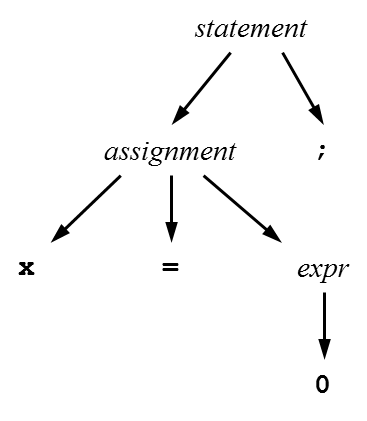
\includegraphics[width=\textwidth]{images/kapitel4/parseTreeGraph.png}
            \caption{Parse-Tree}
            \label{fig:bsp_disp_l}
        \end{subfigure}
        \begin{subfigure}[b]{0.30\textwidth}
            \centering
            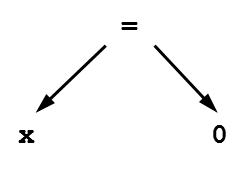
\includegraphics[width=\textwidth]{images/kapitel4/astGraph.png}
            \caption{AST}
            \label{fig:bsp_disp_r}
        \end{subfigure}
        \caption{Parse-Tree und AST der Anweisung \texttt{x = 0;}. Nachgezeichnet aus \cite{book:parrLang}.}.
	    \label{fig:Beispiel_Disparitätsbild}
\end{figure}

Der große Vorteil des AST gegenüber dem Parse-Tree ist die Unabhängigkeit von der Syntax der Sprache. Das bedeutet, dass der AST und auch  nachfolgende Verarbeitungsschritte, die auf dem AST operieren, sich nicht ändern, wenn eine Umbenennung einer Regel in der Sprache vorgenommen wird. Außerdem kann der AST schneller als der Parse-Tree durchlaufen werden, weil die Anzahl der Knoten niedriger ist. Allerdings kann der abstrakte Syntax-Baum nicht vollautomatisch aus dem Parse-Tree generiert werden, sondern nur mithilfe von Regeln, die der Kenntnis der Sprach-Semantik bedürfen und diese widerspiegeln.

\section{Implementierung und verwendete Datenstrukturen}\label{ssct:4.3:implementierung}
Die im Abschnitt \ref{sct:4.2:datenstrukturen} beschriebenen Datenstrukturen kommen - so oder in ähnlicher Form - im Rahmen dieser Abschlussarbeit vor. Ihre Implementierung und Verwendung werden in den folgenden Abschnitten detailliert beschrieben. Abbildung \ref{fig:komponenten} soll einen Überblick über die einzelnen Komponenten und ihr Zusammenspiel geben:

\begin{figure}[H]
\centering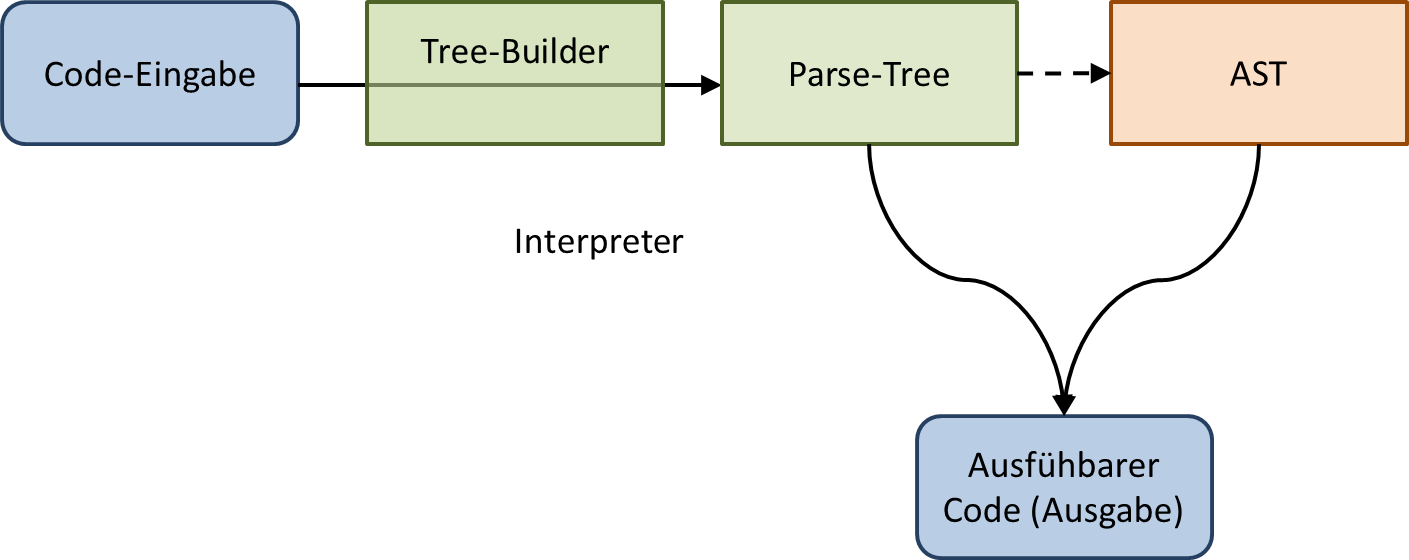
\includegraphics[width=.8\textwidth]{images/kapitel4/komponenten.png}
\caption{Komponenten der internen DSL}
\label{fig:komponenten}
\end{figure}

Die von Abschnitt \ref{ssct:4.3.1:grammatik} bis \todo{Ende} beschriebenen Implementierungen sind ein Ergebnis dieser Abschlussarbeit. Sie werden in der Reihenfolge beschrieben, in der ein Sprach-Ausdruck verarbeitet wird. Abschnitt \todo{Referenz} beschreibt alternativ mögliche Implementierungen.\\
Alle nachfolgend beschriebenen Codebeispiele der Implementierung beziehen sich auf eine DSL für arithmetische Ausdrücke, genannt \textquotedblleft Expression\textquotedblright. Mit ihr lassen sich Rechnungen in den vier Grundrechenarten (\texttt{plus()}, \texttt{minus()}, \texttt{times()}, \texttt{divided}). Das erste Element eines Ausdrucks wird mit der Methode \texttt{expr()} gefasst, um eine Infix-Notation zu ermöglichen. Ihre Grammatik wird nachfolgend näher beschrieben.

\subsection{Definition einer Grammatik durch Interfaces}\label{ssct:4.3.1:grammatik}
Der erste Schritt bei der Implementierung einer Sprache ist das Festlegen der Grammatik. Sie beschreibt durch Regeln, wie ein Strom von Zeichen in einen Syntax-Baum umgewandelt wird \cite{book:fowlerDSL}. Die Grammatik soll, wie in \ref{sct:2.3:ziel} erwähnt, nur durch Interfaces festgelegt werden. Dabei soll es, wie in Abschnitt \ref{ssct:4.1.3:scoping} beschrieben, möglich sein, bestimmte Aufrufreihenfolgen festzulegen.\\ Eine in der EBNF formulierte Grammatik kann äquivalent als Flussdiagramm dargestellt werden. Anhand dieses Flussdiagramms können die dazugehörigen Interfaces folgendermaßen erstellt werden (übernommen und leicht abgeändert von \cite{www:jooq:fluentAPI}):

\begin{itemize}
	\item Jedes Schlüsselwort der DSL ergibt eine Java-Methode
	\item Jede Verbindung ergibt ein Interface
	\item Hat man die Wahl zwischen mehreren Schlüsselwörtern, ohne dass es die Möglichkeit gibt, diese zu überspringen, werden alle diese Schlüsselwörter Methoden in \emph{einem} Interface.
	\item Gibt es ein Schlüsselwort, das wiederholt werden kann, dann hat die Methode, die aus diesem Schlüsselwort resultiert, als Rückgabewert den Typ ihr eigenes Interfaces und nicht den des nächsten.
	\item Kann das nächste Schlüsselwort optional ausgelassen werden, erweitert das aktuelle Interface das Interface mit jenem Schlüsselwort.
	\item Für Schlüsselwörter, die entweder ausgelassen oder genau einmal verwendet werden können, ist Abschnitt \todo{Ref generator-Teil} zu beachten.
	\item Um Rekursion zu ermöglichen, haben betroffene Methoden den Objekt-Typ des Ergebnisses eines Ausdrucks als Parameter. \emph{Bemerkung:} Vollständige Unabhängigkeit zwischen einer Grammatik und ihrer Implementierung kann nur erreicht werden, wenn das Ergebnis eines Ausdrucks in der Sprach-Definition ein generischer Typ-Parameter ist. Aus zeitliche Gründen wurde in dieser Abschlussarbeit auf diesen Schritt verzichtet, da er die Komplexität des Generators (siehe Kapitel \ref{chp:5:automatisierung}) erheblich erhöht. Stattdessen wurde der Typ \emph{ParseTree} (siehe auch Abschnitt)
\end{itemize}

\begin{lstlisting}[caption={Grammatik der Expression-DSL, spezifiziert in EBNF},label=lst:grammar]
	Expression ::= expr '(' ([0-9]+ | Expression) ')'
	               (
	                    plus '(' ([0-9]+ | Expression) ')'
	                  | minus '(' ([0-9]+ | Expression) ')'
	                  | times '(' ([0-9]+ | Expression) ')'
	                  | divided '(' ([0-9]+ | Expression) ')'
	                )*
\end{lstlisting}

\begin{figure}[H]
\centering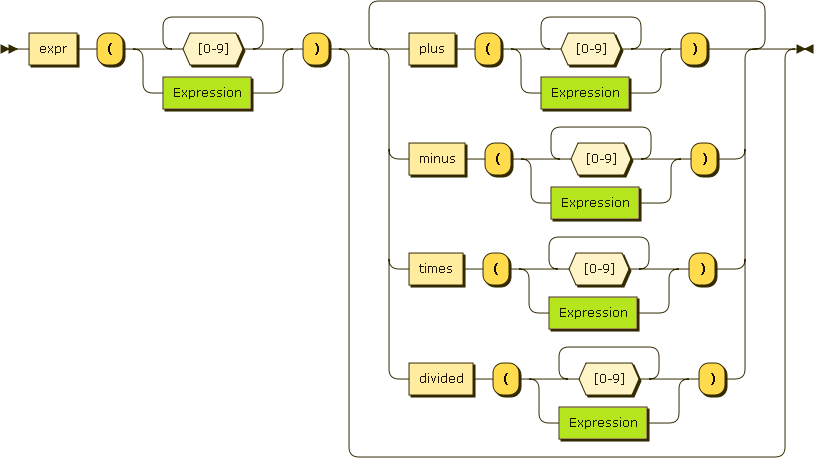
\includegraphics[width=.8\textwidth]{images/kapitel4/expressionRailroad.png}
\caption{Syntax-Diagramm der DSL}
\label{fig:railroad}
\end{figure}

Beispiel-Code

\subsection{TreeBuilder und Scopes}\label{ssct:4.3.2:treebuilder}
Damit die Methoden der durch die Interfaces definierten Grammatik aufgerufen werden können, müssen die Interfaces implementiert werden. Mithilfe von Object Scoping (siehe Abschnitt \ref{ssct:4.1.3:scoping}) wird die gewünschte Aufrufreihenfolge der Methoden festgelegt. Dazu implementiert eine Klasse \textbf{\texttt{C}} jeweils die Methoden eines Interfaces \textbf{\texttt{I}}, inklusive der Methoden derjenigen Interfaces, die \textbf{\texttt{I}} erweitert. Der Inhalt der Methoden dient allein dem Aufbau der Parse-Tree-Struktur (siehe auch: Abschnitt \ref{ssct:4.3.3:parsetree}) und hat keinen semantischen Inhalt. Jede der genannten Klassen - im Folgenden auch speziell Scope-Klassen genannt - hat einen privaten Konstruktor. Dadurch wird verhindert, dass unkontrolliert ein Objekt dieser Klasse instantiiert wird, wodurch die Aufrufreihenfolge verletzt werden könnte.\\
Der Zugriff auf diese Klassen und deren Methoden erfolgt über eine Builder-Klasse, in die alle Scope-Klassen als innere Klassen eingebettet werden. Diese Klasse hält eine private Instanz jeder Scope-Klasse, welche in ihrem Konstruktor erstellt wird. Jede Methode gibt entsprechend der festgelegten Aufrufreihenfolge das Scope-Objekt zurück, welches die nächste erlaubte(n) Methode(n) enthält. Auch der Konstruktor der äußeren Klasse ist privat, da eine Instanz dieser Klasse für einen User keinen Nutzen hat - alle Felder und inneren Klassen sind privat.\todo{Pattern?} Stattdessen erfolgt der Zugriff über eine statische Methode (auch Einstiegsfunktion genannt; im Beispiel: \texttt{begin()}), welche gleichzeitig den Beginn eines jeden Ausdrucks der DSL markiert. Sie ruft den Konstruktor der äußeren Builder-Klasse sowie den derjenigen inneren Klasse mit der ersten Methode auf. Sie gibt das zuletzt erstellte Objekt zurück. Danach kann die erste Methode der DSL aufgerufen werden, usw. Codeausschnitt \ref{lst:treebuilder1} zeigt beispielhaft den Code für eine Builder-Klasse.

\begin{lstlisting}[caption={Code für eine Builder-Klasse mit inneren Scope-Klassen},label=lst:treebuilder1]
	public final class TreeBuilder {
		private final OperatorScope operatorScope;
		
		// privater Konstruktor
		private ExprDSLTreeBuilder() {
			this.operatorScope = this.new OperatorScope();
		}
		
		// Einstiegs-Funktion
		public static StartScope begin() {
			return new ExprDSLTreeBuilder().new StartScope();
		}
		
		// Scope zum Interface "Start"
		public final class StartScope implements Start {
	
			private StartScope() {
			}
	
			@Override
			public OperatorScope expr(final double value) {
				// Code	
			}
			
			// ...
		}
		
		// Scope zum Interface "Operator"
		public final class OperatorScope implements Operator {
			// ...
		}
	}
\end{lstlisting}

Von der Scope-Klasse, welche die erste(n) Methode(n) eines Ausdrucks der DSL enthält, wird kein Objekt in der äußeren Klasse benötigt, da bereits die Einstiegsfunktion das entsprechende Objekt zurückgibt.

Die durch diese Implementierung erreichte Methoden-Verkettung in der DSL bringt den Nachteil des sogenannten \emph{finishing problem} \cite{book:fowlerDSL} mit sich. Es besagt, dass der Methoden-Kette ohne weitere Zusätze ein klarer End-Punkt fehlt. Ohne ihn bleibt ein Ausdruck immer unvollendet und kann nicht weiterverarbeitet werden. Es gibt mehrere Möglichkeiten, dieses Problem zu lösen. In der Implementierung dieser Abschlussarbeit wird eine abschließende Methode verwendet, die ein ParseTree-Objekt des entsprechenden Ausdrucks zurückliefert. Andere Möglichkeiten werden unter Abschnitt\todo{Referenz} beschrieben. Diese Methode - hier \texttt{end()} genannt - wird in einem eigenen Interface platziert.\\
Die Implementierung dieser Methode sowie die vollständige Implementierung der TreeBuilder-Klasse werden im nächsten Abschnitt (\ref{ssct:4.3.3:parsetree}) im Zusammenhang mit der Syntax-Baum-Struktur erklärt.

\subsection{Parse-Tree}\label{ssct:4.3.3:parsetree}
Bei dieser Implementierung handelt sich um eine abgewandelte Form eines Syntax-Baums. Sie ist an DSLs angepasst, die in der Art entworfen wird, welche in dieser Abschlussarbeit vorgeschlagen werden. In der Datenstruktur des Parse-Tree werden, hierarchisch angeordnet, Scope- und Methoden-Knoten gespeichert, wobei Methoden-Knoten demjenigen Scope-Knoten zugeordnet ist, in dem die entsprechende Methode im TreeBuilder steht. Ein Parse-Tree-Objekt kann beliebig viele Scope-Knoten enthalten und ein Scope-Knoten beliebig viele Methoden-Knoten (sofern die Grammatik dies erlaubt). Abbildung \ref{fig:parse-tree} verdeutlicht den Aufbau der Datenstruktur:

\begin{figure}[H]
\centering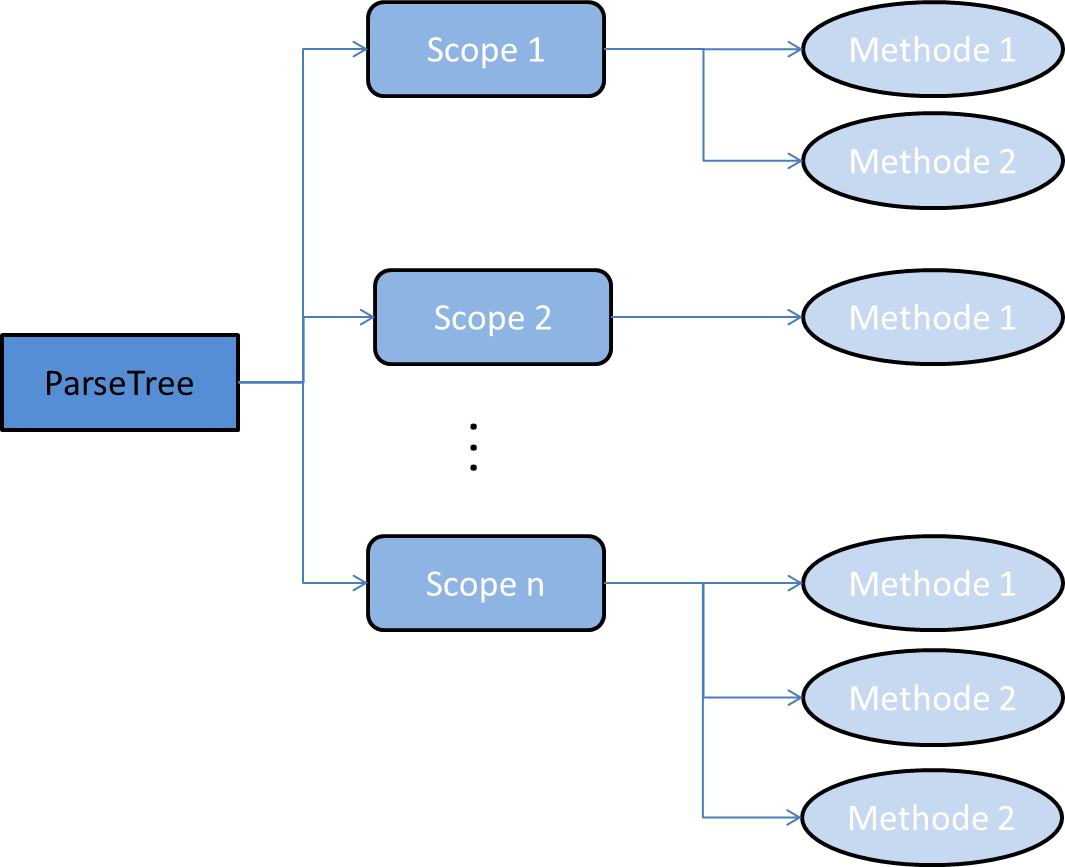
\includegraphics[width=.8\textwidth]{images/kapitel4/parseTree.png}
\caption{Komponenten der internen DSL}
\label{fig:parse-tree}
\end{figure}

Zu jeder Methode der DSL gibt es eine Methoden-Knoten-Klasse. Sie beinhaltet
Jede Methode kann nur einen Parameter haben. Dies erhöht in den meisten Fällen die Lesbarkeit der DSL und eliminiert gleichzeitig die Möglichkeit, Parameter einer Methode zu verwechseln.

Analog dazu


Die Konstruktion eines Parse-Tree-Objekts geschieht durch die Tree-Builder-Klasse: Wird eine Methode aufgerufen, erstellt sie einen Methoden-Knoten mit ihrem Namen und Parameter.

\begin{lstlisting}[caption={Code für eine Builder-Klasse mit inneren Scope-Klassen},label=lst:treebuilder1]
	public final class SimpleMethodNodePlus {
	
		private final String name;
		private final double value;
		
		public SimpleMethodNodePlus(final String methodName, final double val) {
			name = methodName;
			value = val;
		}
	
		public final double getValue() {
			return value;
		}
		
		@Override
		public final String toString() {
			return getName() + '(' + value + ").";
		}
	
	}
\end{lstlisting}

\subsection{Aufbau des Parse-Trees durch den TreeBuilder}\todo{label}

\section{Alternative Implementierungen}

\subsection{AST}\label{sct:4.3.4:ast}
%Danach:
%AST erwähnen
%nochmal erklären, warum Aufteilung in Grammatik, TreeBuilder, ParseTree (und AST) Vorteile mit sich bringt.
%Note, it is possible to model the above DSL with classes instead of interfaces, as well. But as soon as
%you want to reuse similar keywords, multiple inheritance of methods may come in very handy and
%you might just be better off with interfaces.

	% -------------------------------------------------------------------
% Masterarbeit
% Kapitel 5: Automatisierung der Implementierung
% Autor: Daniel Fritz
% Datum: 30.04.2016
% -------------------------------------------------------------------

\chapter{Automatisierung der Implementierung}\label{chp:5:automatisierung}
Dieses Kapitel behandelt die automatische Generierung von Teilen einer internen-DSL-Implementierung anhand einer gegebenen Grammatik in Form von Interfaces, wie sie in Abschnitt \ref{ssct:4.3.1:grammatik} beschrieben wird.\\
Zunächst wird die Template-Sprache \emph{StringTemplate} vorgestellt, die in dieser Abschlussarbeit zur Codegenerierung verwendet wird, danach die Codegenerierung selbst.

\section{StringTemplate}\label{sct:5.1:st}
StringTemplate \cite{www:stringtemplate} ist eine Template-Sprache, die von Terence Parr entwickelt wurde. Gegenüber anderen Template-Sprachen bietet sie eine vollständige Trennung von einem Modell und dessen Präsentation. Die Template-Engine ist einfach in ein Projekt einzubinden\\todo{mehr},
Lückentext, der an den dafür vorgesehen Stellen mit Attributen gefüllt wird
kann:
Eigenschaften auslesen
andere templates aufrufen
listen iterieren


\section{Codegenerierung}\label{sct:5.2:codegenerierung}
In diesem Abschnitt werden automatisch generierbaren Teile der Sprache sowie der Aufbau des Generators erläutert.

\subsection{Generierte Elemente}\label{ssct:5.2.1:generiertes}
Große Teile der in Abschnitt \ref{sct:4.3:implementierung} besprochenen Implementierung können anhand der in Form von Interfaces gegebenen Informationen automatisch erzeugt werden. Die Regeln dafür wurden in Kapitel \ref{chp:4:implementierungstechniken} bereits teilweise genannt. Alle weiteren Informationen, die benötigt werden, sind in Abschnitt \ref{ssct:5.2.2:generator} beschrieben.
Nachfolgend ist eine vollständige Auflistung aller Teile einer DSL-Implementierung, die aus vorgegebenen Interfaces, welche die Grammatik definieren, generiert werden.
\\ \\ %---------------------------------------------------------------
Die \textbf{Tree-Builder-Klasse} inklusive ihrer inneren Scope-Klassen kann nach folgenden Regeln automatisch generiert werden:

\begin{itemize}
	\item Für jedes Interface, das nicht von einem anderen Interface erweitert wird, wird eine Scope-Klasse generiert. Sie besitzt einen privaten Konstruktor und eine private Liste von Methoden-Knoten. Der Name der Scope-Klasse wird nach dem Schema <Interface-Name>Scope festgelegt.
	\item Jede Methode in den Interfaces resultiert in einer Methode in der entsprechenden Scope-Klasse. Allen Methoden ist gemein, dass sie ein entsprechendes Methoden-Knoten-Objekt erstellen und es in der Liste des Scopes ablegen. Davon abgesehen muss unterschieden werden, ob nach Aufruf der Methode im aktuellen Scope verblieben wird, ob er verlassen wird, oder ob das Ende eines Sprach-Ausdrucks erreicht ist.
	\item Die äußere Klasse besitzt ein privates Scope-Objekt für jede vorhandene innere Klasse außer für diejenige, welche die erste Methode eines Ausdrucks enthält. Außerdem hat sie einen privaten Konstruktor, eine private Liste von Scope-Knoten und die Einstiegs-Methode, die das Scope-Objekt mit der (/den) ersten Methode(n) eines Ausdrucks zurückgibt.
\end{itemize}

Für den Namen der Klasse gilt das Schema <DSL-Name>TreeBuilder

\noindent
Pro Scope-Klasse wird auch eine \textbf{Scope-Knoten-Klasse} generiert. Im Konstruktor wird der Name des Scopes eingefügt. Der Name der Klasse ergibt sich aus dem Schema ScopeNode<Interface-Name>.
\\ \\
\noindent
Pro Methode wird eine \textbf{Methoden-Knoten-Klasse} generiert.
Der Name der Klasse ergibt sich aus dem Schema <Methoden-Typ>MethodNode<Interface-Name>. Im Konstruktor wird der Name der Methode eingefügt. Der Methoden-Typ ist entweder \emph{Simple}, \emph{Nested} oder er ist leer.
\\ \\
\noindent
Eine abstrakte Oberklasse für alle Visitor-Implementierungen dieser DSL wird generiert. Sie erbt von \texttt{AVisitor} und enthält leere Implementierungen der visit-Methode für alle Scope- und Methoden-Knoten. Dies ermöglicht eine leichtere Implementierung von konkreten Besuchern, da bereits vorgegeben ist, welche Methoden implementiert werden können. Der Name der Klasse ist durch das Schema A<DSL-Name>Visitor festgelegt.
\\ \\
Für alle generierten Klassen müssen zusätzlich noch korrekte Paket-Definitionen und benötigte import-Statements generiert werden.

\subsection{Aufbau des Generators}\label{ssct:5.2.2:generator}
Der Generator muss alle nötigen Informationen aus den Grammatik-Interfaces extrahieren, und sie für die Code-Generierung an die Templates weitergeben.

Die Codegenerierung umfasst vier Schritte:

\textbf{1. Interfaces analysieren:} Mittels Java Reflection werden alle Interfaces eines vom User spezifizierten Paketes analysiert. Zunächst wird nur festgehalten, welche Interfaces andere erweitern und welche umgekehrt von anderen erweitert werden.

\textbf{2. Informationen auslesen:} Aus den Interfaces werden alle für die Codegenerierung relevanten Informationen ausgelesen und in einer Datenstruktur ähnlich der des \texttt{ParseTree} gespeichert: Ein \emph{\texttt{GeneratorScope}}-Objekt alle nötigen Informationen um Scope- und ScopeNode-Klassen zu generieren. Die GeneratorScope-Klasse hält eine Liste von \emph{\texttt{GeneratorMethod}}-Objekten, welche wiederum die Informationen zum Generieren von MethodNode-Klassen und von Methoden im TreeBuilder enthalten. Informationen aus beiden Klassen gehen in die abstrakte Visitor-Oberklasse ein. Beide Generatorklassen enthalten auch einige Methoden, die nur innerhalb von Templates benötigt werden.

\textbf{3. Überprüfen:} Bei der Verwendung

\subsection{Aufbau der Templates?}
	% -------------------------------------------------------------------
% Masterarbeit
% Kapitel 6: Ergebnis
% Autor: Daniel Fritz
% Datum: 01.05.2016
% -------------------------------------------------------------------

\chapter{Anwendung der Implementierung}\label{chp:6:ergebnis}
Um die im Rahmen dieser Anschlussarbeit entstandene Implementierung nützen zu können, benötigt man die folgenden Pakete:

\begin{itemize}
	\item \textbf{language-package:} Ein Paket mit allen Interfaces, welche die Grammatik der DSL definieren. Der Name des Pakets ist frei wählbar und gibt der DSL ihren Namen.
	\item \textbf{generator:} Ein Paket mit allen Klassen, die für die Codegenerierung nötig sind.
	\item \textbf{main:} Ein Paket, das die Klasse mit der Main-Methode enthält. Dieses Paket ist nicht zwingend notwendig und wird nicht generiert. Das Ablegen der Klasse mit main-Methode schafft hier nur eine bessere Übersicht.
	\item \textbf{parseTree:} Ein Paket, dass alle nicht-generierten Klassen enthält, die im Zusammenhang mit dem Syntax-Baum stehen. Dies sind die abstrakten Baumknoten-Oberklassen \texttt{AMethodNode}, \texttt{ASimpleMethodNode},\\ \texttt{ANestedMethodNode}, \texttt{AScopeNode}, das Interface \texttt{Visitable} und die Klasse \texttt{ParseTree}.
	\item \textbf{templates:} Ein Paket mit allen Template-Dateien, die für die Code-Generierung verwendet werden.
	\item \textbf{visitor:} Ein Paket mit der abstrakten Oberklasse \texttt{AVisitor}. Dies ist auch ein geeigneter Ort für alle konkreten Visitor-Implementierungen.
\end{itemize}

\noindent
Durch das Ausführen der Methode GeneratorMain.main() wird die Codegenerierung  gestartet.
Nach erfolgreicher Generierung stehen folgende Pakete zur Verfügung:

\begin{itemize}
	\item \textbf{parseTreeGen:} Ein Paket, das alle generierten Baumknoten-Klassen enthält. Des weiteren enthält es die generierte TreeBuilder-Klasse.
	\item \textbf{visitorGen:} Ein Paket mit der generierten abstrakten Oberklasse aller konkreten Visitors dieser DSL.
\end{itemize}

\section{Hinweise zur Anwendung}\label{sct:6.1:hinweise}
Abgesehen von der Definition der DSL-Grammatik durch Interfaces benötigt der Code-Generator folgende Informationen vom User:

\begin{itemize}
	 \item Den relativen oder absoluten Pfad zum Paket, in dem alle Grammatik-Interfaces liegen. Der Name des Pakets ist gleichzeitig auch der Name der internen DSL.
	 \item Den Pfad, unter dem die generierte TreeBuilder-Klasse und alle generierten Baum-Knoten-Klassen gespeichert werden sollen.
	 \item Den Pfad, unter dem die generierte abstrakte Visitor-Oberklasse gespeichert werden soll.
	 \item Anmerkung: Bei beiden Pfaden sind keine sub-packages erlaubt.
	 \item den Namen des Interfaces, das die erste(n) Methode(n) eines DSL-Ausdrucks enthält.
\end{itemize}

\noindent
Außerdem müssen die folgenden Einschränkungen beachtet werden:

\begin{itemize}
	\item Alle Grammatik-Interfaces müssen einen eindeutigen Namen haben. Zusätzlich müssen die Namen mit einem Großbuchstaben beginnen. Obwohl beides meist erzwungen wird, sei der Hinweis an dieser Stelle gegeben.
	\item Pro Methode ist höchstens ein Parameter erlaubt. Grundsätzlich ist es natürlich möglich, Methoden mit mehreren Parametern in einer DSL zu haben. Jedoch birgt es die Gefahr in sich, dass die Parameter versehentlich vertauscht werden oder der Charakter einer flüssig lesbaren Sprache verloren geht. Darum wurde diese Einschränkung bewusst vorgenommen.
	\item Mindestens eine Methode der Sprache muss den Rückgabewert \texttt{ParseTree} haben. Ansonsten kann kein Ausdruck der Sprache vervollständigt werden.
	\item In allen Grammatik-Interfaces darf es keine zwei \emph{gleichen} Methoden geben. Zwei Methoden werden in dieser Implementierung als \emph{gleich} erachtet, wenn ihr Name übereinstimmt und beide Methoden entweder den Parameter \emph{ParseTree} oder beide nicht den Parameter \texttt{ParseTree} haben. In diesem Fall würden beide Methoden mit demselben Methoden-Knoten im ParseTree abgebildet und würden von derselben \texttt{visit}-Methode besucht.
	\item Es dürfen keine generischen Typ-Parameter verwendet werden.
\end{itemize}
	% -------------------------------------------------------------------
% Masterarbeit
% Kapitel 7: Fazit
% Autor: Daniel Fritz
% Datum: 04.05.2016
% -------------------------------------------------------------------

\chapter{Fazit und Ausblick}\label{chp:7:fazit}
In dieser Masterarbeit sollten folgende Ziele erreicht werden:

Ziel dieser Masterarbeit war die teilweise automatische Implementierung interner Java-DSLs. Grundlage einer Sprache sind dabei Interfaces, welche die Grammatik der Sprache definieren. Es sollte eine möglichst strikte Trennung der Komponenten der Implementierung untereinander erreicht werden. Verbunden damit war die Frage, ob diese (Generierung) den Entwicklungsprozess einer DSL verkürzen bzw. vereinfachen kann.

In den folgenden Abschnitten werden die Ergebnisse dieser Arbeit zusammengefasst. Zudem wird ein Ausblick auf künftige Entwicklungen gegeben.

\section{Ergebnisse}\label{sct:7.1:ergebnisse}
Die erste Phase dieser Abschlussarbeit bestand aus der manuellen Implementierung einer internen Java-DSL anhand einer einfachen Sprache für arithmetische Ausdrücke. In mehreren Iterations-Schritten wurden den Anforderungen genügende Daten-Strukturen entwickelt, die in Kapitel \ref{chp:4:implementierungstechniken} beschrieben sind.
Dabei spielte die Unabhängigkeit der Definition einer Sprache von ihrer Implementierung und die klare Trennung der Komponenten untereinander eine wichtige Rolle.

In der zweiten Phase 

\section{Ausblick}\label{sct:7.2:ausblick}
	
	%\bibliographystyle{plain} % autor, jahr
	\printbibliography

\end{document}

